\section{Postflop Strategy}
Reaching the flop means we have access to more information that enables us to conceptualize how the hand will progress. Usually, as the round progress, the number of active opponents decreases, making it easier to estimate the strength of our hand. In the next section, we will explore how PokerShark estimates the strength of its pocket.

\subsection{Hand Strength}
We need to define a metric that enables us to assess how our pocket would perform against the hands of the opponents. Numerous methods were proposed in the literature, such as Artificial Neural Networks\cite{bensson2013predicting}, Monte Carlo analysis, and enumeration \cite{billings_challenge_2002}.

Before discussing hand strength, we need to solve the problem of comparing two hands. There are three community cards on the flop, and each player has two pocket cards, which means a 5-card hand can already be constructed. So if the opponents show their cards, how can we tell which hand is the strongest?

\subsubsection{Absolute Hand Rank}
Comparing hands is not trivial, but it can be done efficiently using the absolute hand rank, which is a numerical value assigned to each possible hand that allows us to compare hand strength.
There are many implementations of the absolute hand rank, but most implementations are based on Cactus Kev's Algorithm\footnote{\url{https://suffe.cool/poker/evaluator.html}}. Although we do not want to go extensively into this topic, we will provide a high-level outline. There are 2.598.960 unique possible hand combinations, but most hands are not distinct. For example, \card{H}{A}\card{D}{A}\card{C}{A}\card{S}{A}\card{H}{K} and  \card{H}{A}\card{D}{A}\card{C}{A}\card{S}{A}\card{D}{K} are unique hands but have the same rank.

If we only consider distinct hands, we have only 7462 different combinations, which is manageable.

% table of distinct hands
\begin{table}[h]
    \centering
    \begin{tabular}{|c|c|c|}
        \hline
        \textbf{Hand Value} & \textbf{Unique}  & \textbf{Distinct} \\\hline
        Straight Flush      & 40               & 10                \\\hline
        Four of a Kind      & 624              & 156               \\\hline
        Full Houses         & 3744             & 156               \\\hline
        Flush               & 5108             & 1277              \\\hline
        Straight            & 10200            & 10                \\\hline
        Three of a Kind     & 54912            & 858               \\\hline
        Two Pair            & 123552           & 858               \\\hline
        One Pair            & 1098240          & 2860              \\\hline
        High Card           & 1302540          & 1277              \\\hline
        \textbf{TOTAL}      & \textbf{2598960} & \textbf{7462}     \\\hline
    \end{tabular}
    \caption{Number of unique and distinct hands}
    \label{tab:unique}
\end{table}

These combinations are ordered into a hash table with an index representing the hand's value. Finally, an encoding function is used to create a hand mask that can be used to look up the hand's value using the hash table. This algorithm enables us to compare hands efficiently, which is a very important tool that we will utilize in estimating hand strength. We have to note here that the following methods and algorithms are heavily influenced by \cite{billings_challenge_2002},\cite{papp_dealing_1998}, and \cite{davidson_improved_2000}.


\subsection{Facing one Opponent}
when facing one opponent post-flop enumerating all his possible pockets is not computationally hard. The deck of cards has 52 cards, we have two cards, and on the flop, we get to see three of the board cards, leaving the opponent with ${47 \choose 2} = 1081$ possible combinations that a modern  CPU can enumerate through in a matter of milliseconds. The number of possible combinations only goes down as the round progress.

\begin{Algorithmus}[H]
    \caption{Hand Strength estimation against one opponent}
    \label{alg:enum}
    \begin{algorithmic}
        \Procedure{HandStrength}{$Pocket, Board$}
        %\State $Wins, Count  \gets 0$
        \State $PocketRank \gets GetAbsoluteHandRank(Pocket | Board)$
        \For {$OpponentHand \in GetPossibleHands(Pocket, Board)$}
        \State $OpponentRank \gets GetAbsoluteHandRank(OpponentHand)$
        \If {$OpponentRank > PocketRank$}
        \State $Wins \gets Wins + 1$
        \EndIf
        \If {$OpponentRank = PocketRank$}
        \State $Wins \gets Wins + 0.5$
        \EndIf
        \State $Count \gets Count + 1$
        \EndFor
        \State \Return $Wins / Count$
        \EndProcedure
    \end{algorithmic}
\end{Algorithmus}

Algorithm \ref{alg:enum} is used to deliver the win odds of our hand by iterating throw all possible opponent hands. We consider a draw as half as good as a win. Although the algorithm might seem very reasonable at first glance, it does not consider opponent preferences, which is a significant weakness because post-flop, almost all of the weak hands have already been folded. Many of the wins we are counting toward hand strength have no value in practice. Let us consider the following board: \card{C}{Q}\card{S}{Q}\card{D}{J}\card{H}{7}\card{D}{3} and the pocket \card{C}{A}\card{D}{K}. The previous algorithm will assume all opponent's hands are equally likely and will give a 0,51 win odds. If we are facing a tight opponent with a range similar to the one shown in figure \ref{fig:tight}, the actual win odds are closer to 0,12 which is a big difference.

\begin{figure}[h]
    \centering
    \includegraphics[width=0.5\textwidth]{tight.png}
    \caption{Tight opponent range}
    \label{fig:tight}
\end{figure}

Here is where adjustment matrices and opponent models prove valuable. We can adjust the algorithm to weigh each win/draw resulting in a much more accurate estimation.

\subsection{Hand Potential}

One very important factor that we need to take into consideration when assessing hand strength is how future board cards are going to affect our pocket. For example, our pocket is \card{H}{8}\card{H}{7} and a board of \card{H}{A}\card{H}{T}\card{S}{3} the direct hand strength of our hand is low 0,18 (assuming the opponent has no preferred range). However, any heart card will give us a flush. With a seven or eight, we can get one or two pairs. Nine and six or Jack and nine will make a straight. The hand has a significant chance to improve with two board cards remaining.

Creating a mathematical notion for hand potential has to include the probability $PP$, the probability of the hand improving from a loss or draw to a win, and $PN$, the probability of the hand worsening going from a win or draw to a loss.

There are three board cards on the flop, and as calculated earlier, the opponent has 1081 possible pockets. The two remaining board cards can be chosen from 45 cards, meaning ${45 \choose 2}$ = 990 possible combinations. In total, we have to enumerate 1081 * 990 = 1.070.190 different cases, which is not challenging for a modern CPU.

On the turn, there are significantly fewer cases to consider, ${46 \choose 2}$=  1035 possible opponent's pockets, and one of 44 cards as a potential board card leaving us with 1035 * 44 = 45.540 cases to consider.

$PP$ and $PN$ are calculated as follows:
$$PP =\frac{P_{loss,win} + \cfrac{P_{loss,tie}}{2} + \cfrac{P_{tie,win}}{2}}{P_{loss} + P_{tie}}$$
$$PN =\frac{P_{win,loss} + \cfrac{P_{win,tie}}{2} + \cfrac{P_{tie,loss}}{2}}{P_{win} + P_{tie}}$$

The enumeration can also be weighted using the opponent model to get more accurate estimations. PokerShark uses The \textit{HandPotential} Algorithm, which calculates $PP$ and $PN$. The Algorithm is explained in detail in \cite{papp_dealing_1998}.

\subsection{Facing n Opponents}

Introducing another opponent to the game will dramatically increase the number of combinations and cases we need to enumerate. Adding more opponent will increase the number of the needed enumrations to the point that it is not feasible anymore. To solve this problem, we approximate the odds by calculating the product of the odds facing each opponent separately.
$$W = W_{op1} * W_{op2} * \dots * W_{opn}$$
This approach does not consider the dynamic of the opponents interacting with each other. However, it gives us a simple solution to a complex problem while utilizing the different preferences each opponent has shown. A similar approach is used for the hand potential.


\subsection{Monte Carlo Simulation}
The accuracy of the two algorithms, HandStrength and HandPotential, directly depends on the accuracy of the model. To adjust for any inaccuracy in the modeled preferences of the opponents, we use the result of a Monte Carlo simulation. The simulation uses the same number of opponents that the bot is facing, but it does not take into consideration any preferences. The results of the simulation are then used to adjust our estimation.

\subsection{Hand Strength Estimation}

We combine the previously examined algorithms and methods to get an estimate of the strength of the hand. Since inaccurately profiling the opponent has a significant impact on the algorithm's predictions, we must place a greater emphasis on the simulation result:
$$S = W_n * 0.35 + MCS * 0.65$$
Finally, we add the normalized sum of the hand potential:
$$HS_n = S + (1-S) PP - (S * PN)$$

\subsection{Expected Utility Implementation}
Although FluidHTN has a big community, we could not find any prebuilt solutions for expected utility. Fortunately, FluidHTN is very flexible and easy to extend. We have extended Primitive tasks to include a list of possible utilities with their probabilities and added a new type of Compound tasks called ExpectedUtilitySelector, which decomposes the task with the highest expected utility from the applicable tasks.

\begin{table}[h]
    \centering
    \begin{tabular}{|l|l|l|}
        \hline
        \textbf{Construct}               & \multicolumn{1}{c|}{\textbf{Description}}                                                       \\ \hline
        \textit{VariableUtility}         & Pair of utility an probability.                                                                \\ \hline
        \textit{VariableUtilityTask}     & Extention of PrimitiveTask to include a list of VariableUtility.                                \\ \hline
        \textit{ExpectedUtilitySelector} & Extention of Selector that can have only VariableUtilityTasks as subtasks. \\ \hline
    \end{tabular}
    \caption{Expected Utility Constructs}
\end{table}

\textit{VariableUtilityTask} can calculate its expected utility based on the current risk attitude of the bot. Each one of the attitudes corresponds to a utility function. Figure \ref{fig:utilityfunctions} shows the mathematical functions used to adjust the expected return of each outcome.

\begin{figure}[h]
    \centering
    \begin{subfigure}[b]{0.33\textwidth}
        \centering
        $$U(c)= - \frac{e^{-\alpha c} -1}{\alpha}$$
        \caption{Risk Averse}
        \label{fig:riskaverse}
    \end{subfigure}
    \begin{subfigure}[b]{0.33\textwidth}
        \centering
        $$U(c)= c$$
        \caption{Risk Neutral}
        \label{fig:riskneutral}
    \end{subfigure}
    \begin{subfigure}[b]{0.33\textwidth}
        \centering
        $$U(c)= \frac{e^{\alpha c} -1}{\alpha}$$
        \caption{Risk Seeking}
        \label{fig:riskseeking}
    \end{subfigure}
    \caption{Utility Functions, Where $\alpha$ is the risk sensitivity}
    \label{fig:utilityfunctions}
\end{figure}

\textit{ExpectedUtilitySelector} uses the algorithm shown in listing \ref{alg:bestTask} to find the task with the highest utility among the applicable tasks.


\begin{Algorithmus}[H]
    \caption{Find the task with the highest utility}
    \label{alg:bestTask}
    \begin{algorithmic}
        \Procedure{FindBestTask}{$Context, SubTasks$}
            \For {$SubTask \in SubTasks$}
                \If {$SubTask.IsApplicable(Context)$}
                    \State $Utility \gets SubTask.GetUtility(Context)$
                    \If {$Utility > BestUtility$}
                        \State $BestUtility \gets Utility$
                        \State $BestTask \gets SubTask$
                    \EndIf
                \EndIf
            \EndFor
            \State \Return $BestTask$
        \EndProcedure
    \end{algorithmic}
\end{Algorithmus}

The \textit{FindBestTask} Algorithm does not traverse to lower layers of the search tree because the search tree in our use case has only one layer.

\subsection{Decision making}

Although expected utility gives us a great deal of control to guide the decision-making process of the bot, we need other mechanisms to achieve certain behaviors. For example, raising actions involve inherently more risk than folding or calling. Thus the utility of raise actions should be treated differently than the utility of folding or calling. 
Strictly following expected utility would result in a bot that rarely bluffs, which is a very important tactic in Texas Hold'em. Additionally, there is a wide range of tactics that we would like the bot to utilize. One example of such tactics is Slow-Playing, where even when holding a strong hand, the player does not place a big raise but rather performs a series of calls or small raises, setting up a trap for the opponents. 

\begin{figure}[h]
    \centering
    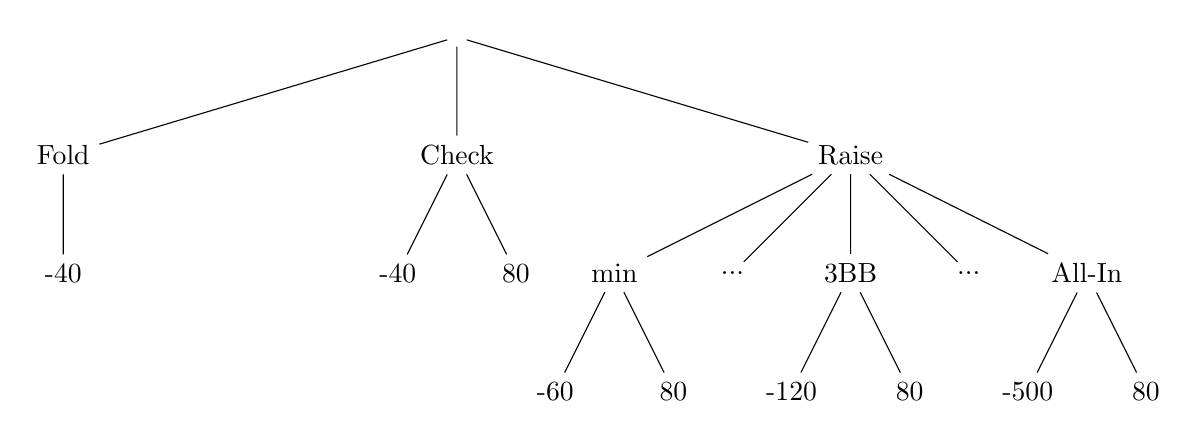
\begin{tikzpicture}
        \node {} [sibling distance = 5cm]
           child {
                node{Fold}
                child{node{-40}}
           }
           child {
                node{Check}[sibling distance = 1.5cm]
                child{node{-40}}
                child{node{80}}
           }
           child {
                node{Raise} [sibling distance = 1.5cm]
                child{node{min} child{node{-60}} child{node{80}}}
                child{node{...}}
                child{node{3BB} child{node{-120}} child{node{80}}}
                child{node{...}}
                child{node{All-In}child{node{-500}} child{node{80}}}
           };
    \end{tikzpicture}
    \caption{Decision Tree without adjusment}
\end{figure}

We solved this problem by introducing an adjustment matrix used to increase or decrease the utility of raises based on the raise amount and hand strength. Figure \ref{fig:adfactors} shows how the raise amount and hand strength affect the adjusment factors. Some rules have also been added to deter the bot from calling when its hand is weak. In addition, some limits on the raise amount have also been implemented in some cases. Finally, we utilized the probabilistic nature of the decision object to prevent premature raises and to shape the bot's behavior to prefer slow playing.

\begin{figure}[h] 
    \centering
    \includegraphics[width=\textwidth/2]{graphics/adfactors.png}
    \caption{Adjustment Factors}
    \label{fig:adfactors}
\end{figure}

